\chapter{硬件模块介绍}

\section{基于FIFO的可变长移位寄存器设计}

\begin{figure}[h]
    \centering
    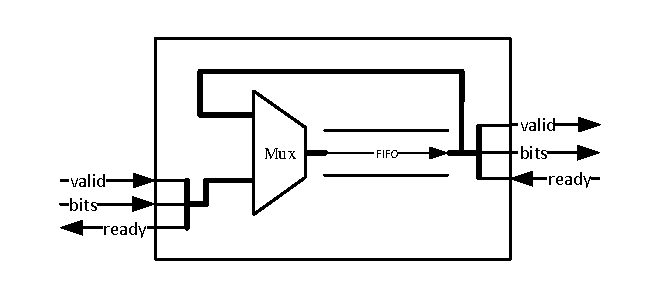
\includegraphics{../pdf/fifoshift.pdf}\\
    \caption{FIFO Shift}
\end{figure}

    \subsection{BRAM与DRAM选择}

\section{SRAM部分在FPGA中的优化}

\section{基于Xilixn 7Series FPGA片上DSP的高性能乘法器}

\section{PE单元构造}

\section{用于数据分发的简易NoC设计}

\section{PE阵列生成器}
    \subsection{计算流程}

\section{顶层接口设计}

\section{本章小结}
% \subsection{二级节标题}

% \subsubsection{三级节标题}

% \paragraph{四级节标题}

% \subparagraph{五级节标题}

% \section{脚注}

% Lorem ipsum dolor sit amet, consectetur adipiscing elit, sed do eiusmod tempor
% incididunt ut labore et dolore magna aliqua. Ut enim ad minim veniam, quis
% nostrud exercitation ullamco laboris nisi ut aliquip ex ea commodo consequat.
% Duis aute irure dolor in reprehenderit in voluptate velit esse cillum dolore eu
% fugiat nulla pariatur. Excepteur sint occaecat cupidatat non proident, sunt in
% culpa qui officia deserunt mollit anim id est laborum.
% \footnote{This is a long long long long long long long long long long long long
% long long long long long long long long long long footnote.}
